\chapter{Introduction}

\section{RoboCup}
The ultimate goal in AI, probably in robotics, is to build intelligent systems capable of displaying complex behaviors to accomplish the given tasks through interactions with a dynamically changing physical world. RoboCup simulation has emerged as an excellent domain for researchers to test ideas in machine learning and extend the reach of AI. In a generation where machines have evolved to beat humans in the game of Chess and Go, learning in the RoboCup soccer domain involves a whole new set of challenges, such as a continuous multi-dimensional state space, noisy sensors, need to cooperate with other agents to form team strategies and the need to act in real-time. Machine learning techniques have been used in the past on a wide range of tasks in RoboCup that include both individual behaviors and team strategies. We explore one such strategy to learn a generic individual behavior. 
\\\\
Reinforcement learning (RL) is an area of machine learning concerned with how software agents ought to take actions in an environment to maximize some notion of a cumulative reward. In context of RoboCup, we try to explore this idea to train soccer bot to learn basic skills like walking and kicking. The current walk of these bots is somewhat unnatural, and we feel that if it is made more human-like then perhaps robots could learn to perform complex tasks like passing and dribbling much more aptly and therefore get one step closer towards achieving human level competence. To make if more human-like, we model the rewards in our reinforcement learning task in such a way that robots try to mimic human motion while accounting for physical forces that act on it.
\\\\
For good rewards, we need motion clips to be based on our robot hierarchy. A skeleton hierarchy is composed of a series of joints and joints chains with hierarchical relationships. Each joint in a skeleton hierarchy is a child joint and a parent joint. A parent joint is any joint higher in a skeleton's hierarchy than any of the other joints that are influenced by that joint's actions. Standard available motion clips are based on their own specific skeleton hierarchy. Transforming these motion clips to fit on our agent's skeleton hierarchy poses a difficult challenge. Motion retargeting deals with this specific problem on a very generic scale. The objective is to adapt an animated motion from one character to another under some physical constraints. In our case, we have to overcome the issue of different joint lengths while simultaneously constraining correct foot placements. 

\begin{figure}
\centering
  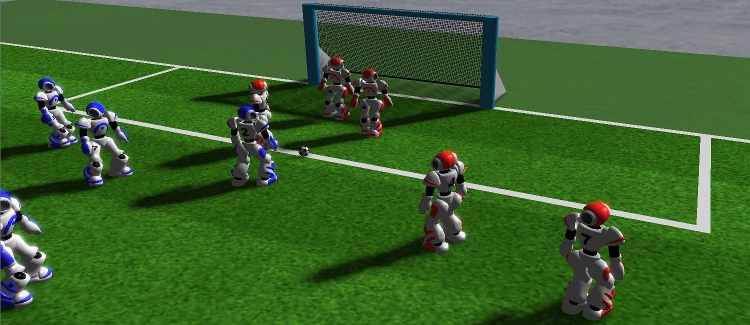
\includegraphics[width=\linewidth]{images/3DRoboCup.jpg}
  \caption{3DRoboCup Simulation with two teams of Red and Blue Nao Agents}
  \label{fig:robocup}
\end{figure}

\\\\
\section{Problem statement}
Under the standard rules of RoboCup Competition \cite{usermanual}, and physical forces like, friction, gravity and others we need to train a standard Nao agent to walk (and perform other basic skills later) smoothly without falling. This process has to be accomplished via training the soccer bots using human motion clips so that the resultant walk is more natural. This requires agent learning to provide a right set of torques to appropriate joints at right time in the simulation. 

\section {Work Partition}
In part 1 of this project, we designed the general framework for training, getting rewards, runnning simulations that essentially enabled us to do testing and experimentation in part 2. The retargeting problem as well as other major server flaws were debugged in part 2.
  
\section{Report Outline}
The rest of this report is organized as follows. In Chapter 2 we outline the existing literature related to our work. Chapter 3 describes the approaches we tried along with the challenges we faced. In Chapter 4 we provide an overview of our implementation framework. We present our results in Chapter 5 followed by conclusion and future extensions in Chapter 6.